\section{Prime monodromy, complete clock observations, and the original
zeta
weights}\label{prime-monodromy-complete-clock-observations-and-the-original-zeta-weights}

24 September 2026. This receives the two identical pasted transcripts
accompanying arxiv-pisa.tex and stack2.png. The transcripts are retained
verbatim, including their tentative formulations; assistant text within
them is not promoted to a user definition. The question investigated
here is the user's proposed common global requirement of infinite
observation, and its relation to arithmetic weight.

The notation Z\_0, Z\_1, Z\_2, \ldots{} continues to mean the user's
absence/presence and quantum-number layers. The symbols Q\_d below name
explicitly constructed d-state winding clocks; they do not silently
redefine the user's entire Z\_d algebra. The distinction between an
absent datum and an existing datum whose observed count is zero remains
throughout. Addition at tau is not restored.

The primary source is Alain Connes and Caterina Consani, \emph{Knots,
primes and class field theory},
\href{https://arxiv.org/abs/2501.06560v1}{arXiv:2501.06560v1}, original
arxiv-pisa.tex. The supplied file is byte-identical to the original
source. Its mapping-torus propositions, finite-cover theorem and
class-field comparison are read directly in TeX. The picture's three
upper components are over ONE prime p.~Their labels are primes above p
in an extension; their vertical drawing positions are not three
successive quantum-number levels. M2 constructs an exact example with
those three components and their winding data.

\begin{figure}
\centering
\pandocbounded{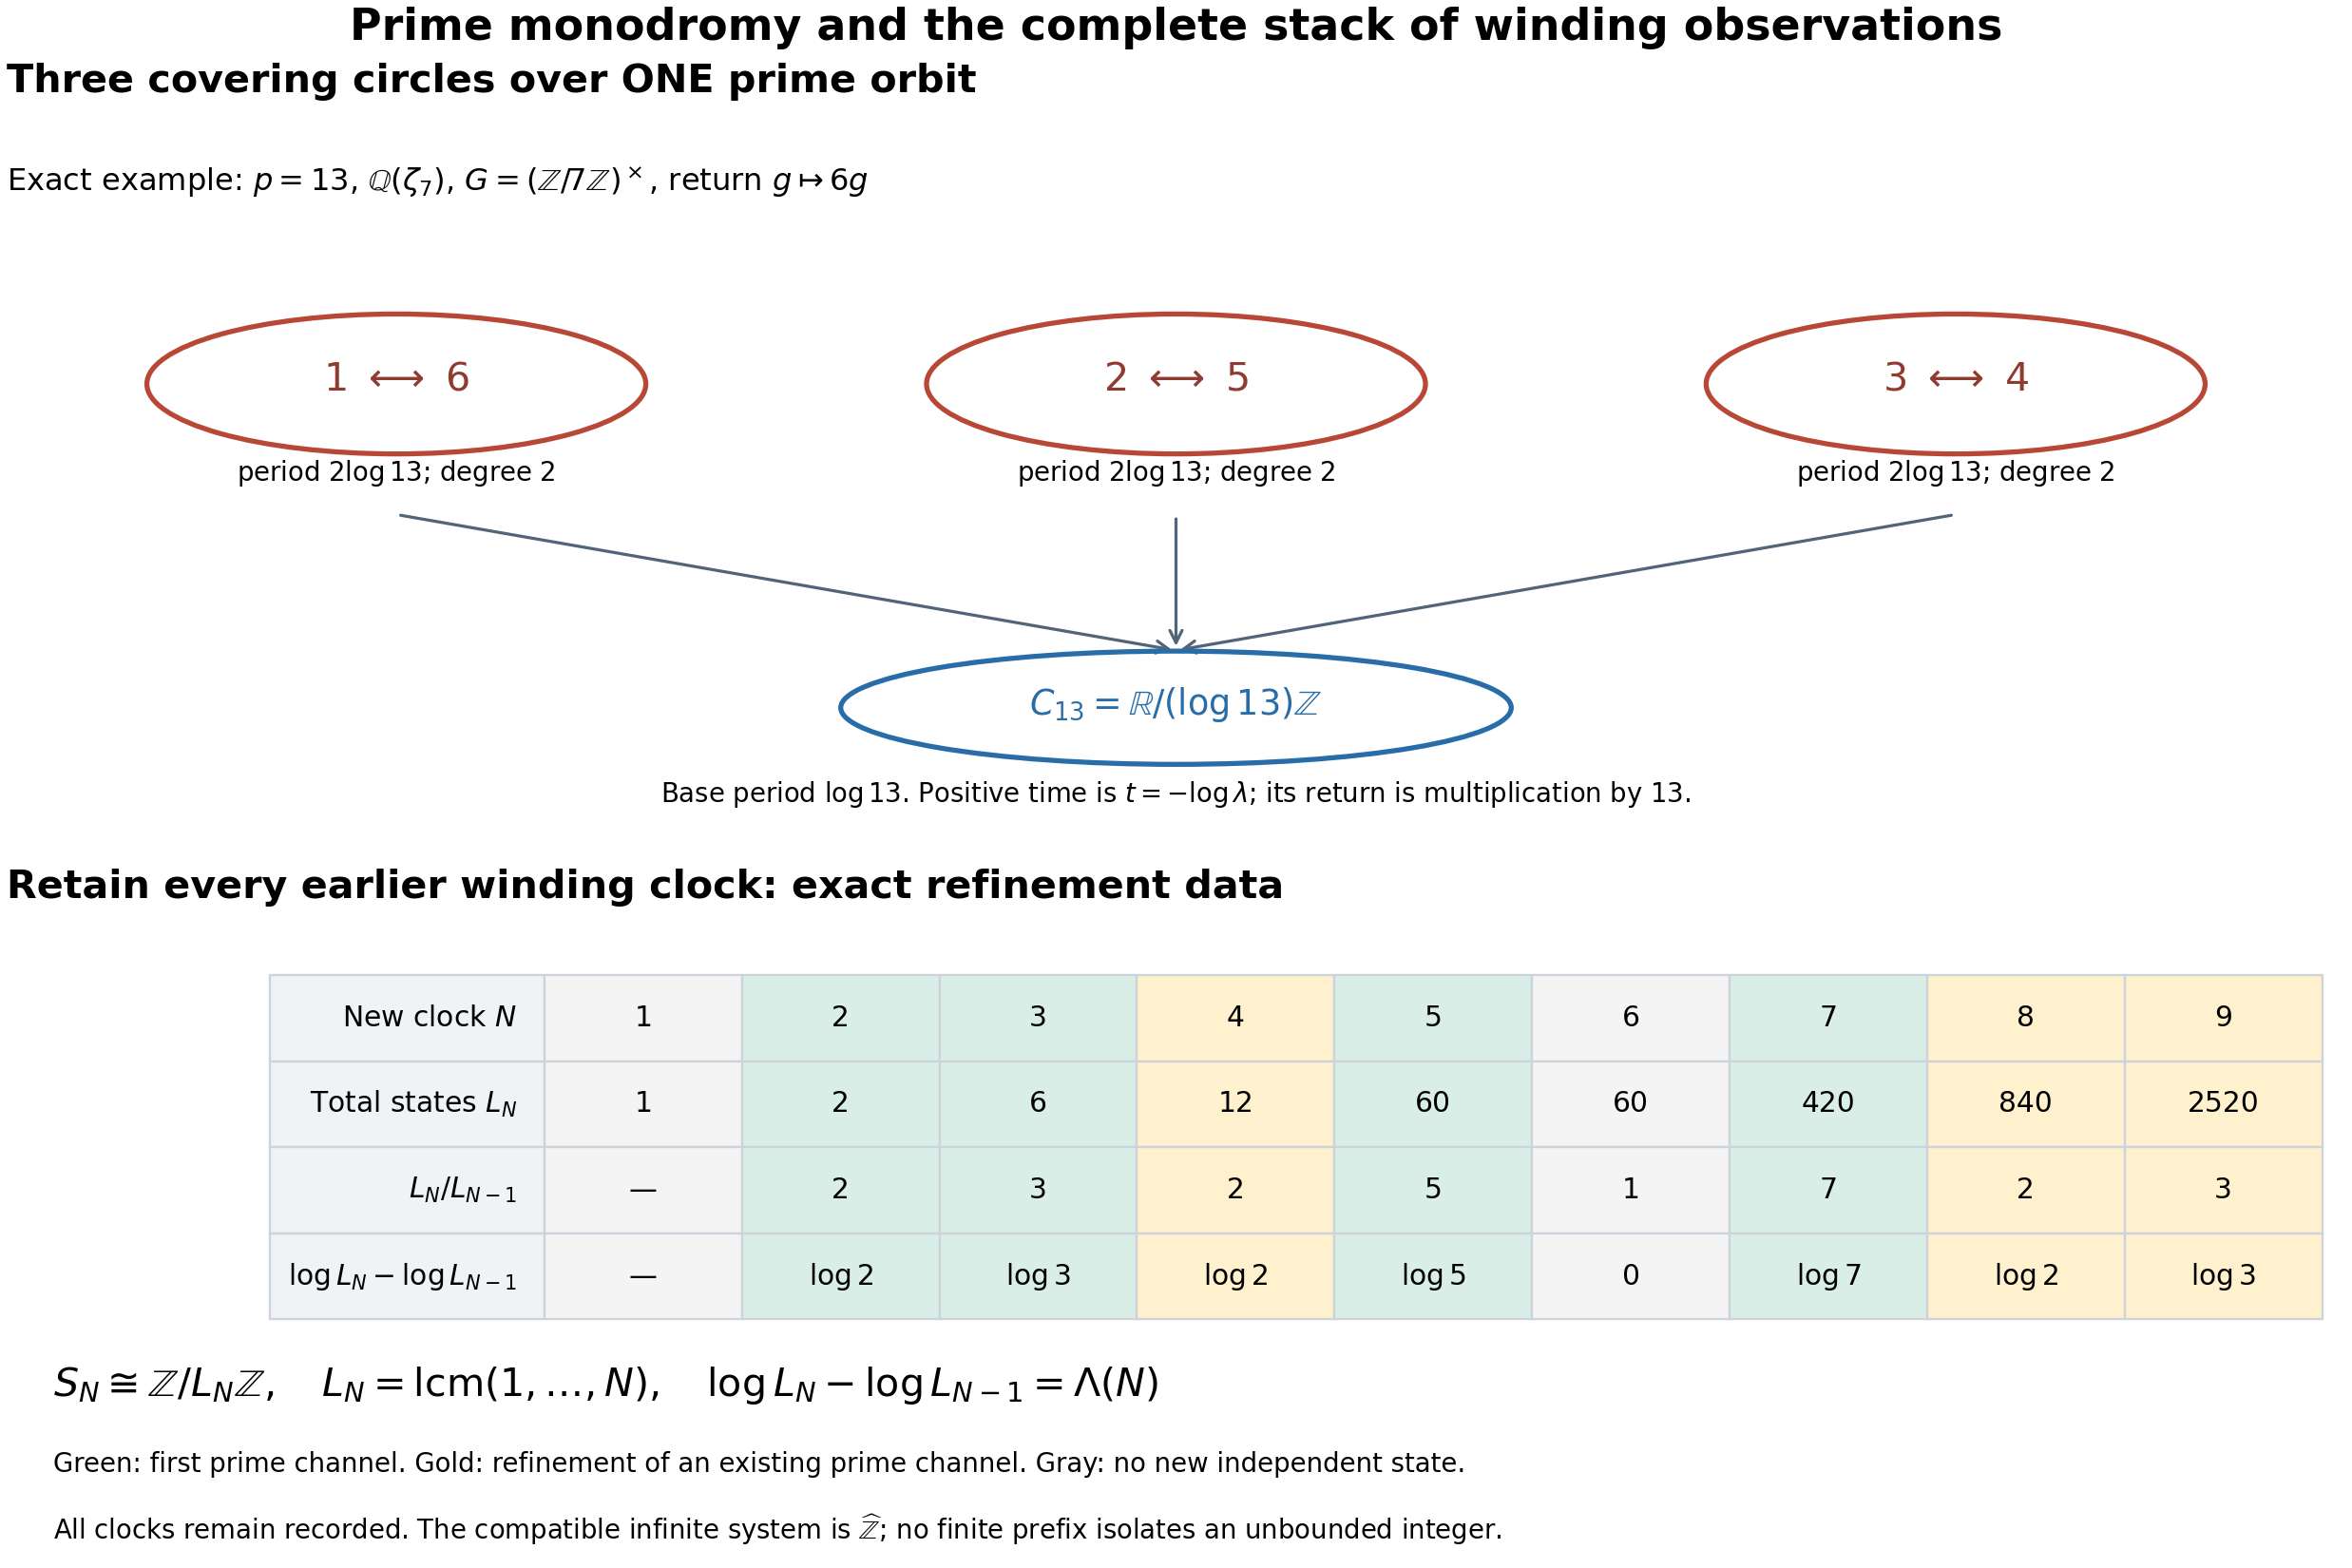
\includegraphics[keepaspectratio,alt={Exact prime cover and complete winding-clock refinements}]{prime_monodromy_history.png}}
\caption{Exact prime cover and complete winding-clock refinements}
\end{figure}

Figure M. Above: the three components for p=13 in Q(zeta\_7), with
return multiplication by 6 modulo 7, covering degree 2 and both real
periods retained. Below: the exact first nine stages of the all-clock
receiver. The all-N argument is M4--M6, not an extrapolation from this
table. The supported original-zeta comparison is M7. Human source:
Connes--Consani, original arxiv-pisa.tex, Proposition mappingtorus and
its finite-cover calculation. Reproducible figure source:
draw\_prime\_monodromy\_history.py; exact displayed data:
MONODROMY\_FIGURE\_CHECKS.json. The drawing is schematic; ellipse sizes
are not a metric on the source base.

\subsection{M1. Presence and a zero reading have an explicit
comparison}\label{m1.-presence-and-a-zero-reading-have-an-explicit-comparison}

Use the actual generic monoid retained in C2 of
TAU\_TWISTOR\_TATE\_AND\_WEIL.md:

\[
A_\eta=\{0\}\cup\{J^rT^m:r\in\mathbb Z/4\mathbb Z,\ m\in\mathbb Z\},
\qquad J^2=\epsilon,\quad J^0T^0=\tau.
\tag{M1.1}
\]

The multiplication adds m, adds r modulo 4, and has absorbing element 0.
Define the presence observation

\[
P:A_\eta\longrightarrow\{0,\tau\},\qquad
P(0)=0,\quad P(J^rT^m)=\tau.
\tag{M1.2}
\]

It is multiplicative because a product of two nonabsorbing elements is
nonabsorbing, and a product with 0 is 0. It is invariant under the
source mirror J\textsuperscript{rT}m -\textgreater{}
J\textsuperscript{(-r+2m)T}(-m). Thus zero accumulated winding m=0 does
not make a present datum absent: the whole fibre m=0 contains
tau,J,epsilon,J\^{}3. The winding projection is defined on the
nonabsorbing group; P is defined on the pointed monoid. These are two
proved maps on the same structure.

This comparison does not settle the user's tentative proposal to rename
eta or the pair Z\_0/Z\_1. The source generic point eta, its stalk
A\_eta and the stalk unit tau have different types, connected by the
stalk's projection to its supporting point and by M1.2. The unit in M1.1
is not identified with integer zero. When an integer count is
represented by an exponent m, retain its count label separately from the
base label tau, including at m=0. Winding-return parity is an
observation on this exponent; it is not an assignment of intrinsic
integer parity to tau.

\subsection{M2. What the supplied stacked picture
represents}\label{m2.-what-the-supplied-stacked-picture-represents}

Fix a rational prime p and put ell\_p=log(p). To avoid collision with
the source's additive group denoted H\_p in FF.tex, write

\[
\mathcal H_p=\prod_{q\ne p}\mathbb Z_q^\times.
\tag{M2.1}
\]

The original Proposition \texttt{mappingtorus} identifies the inverse
image of the prime orbit with

\[
\pi^{-1}(C_p)\cong
(\mathcal H_p\times\mathbb R_{>0})/\big((h,\lambda)\sim(ph,p\lambda)\big),
\quad C_p=\mathbb R_{>0}/p^{\mathbb Z}.
\tag{M2.2}
\]

The retained adelic representative has coordinate h\_q at every q!=p,
coordinate 0 at p, and archimedean coordinate lambda. Multiplication by
a positive rational preserves this form exactly when that rational is a
power of p, because all its valuations outside p must be zero. This
proves the orbit equivalence in M2.2 directly. The full existence and
equivariance are the source proposition, with its representative map
kept here.

For orientation, let t=-log(lambda). Then M2.2 becomes

\[
(h,t+\ell_p)\sim(ph,t).
\tag{M2.3}
\]

Thus a positive t-circuit returns h to ph. A positive
log(lambda)-circuit has inverse return. Both orientations and the
original length ell\_p remain displayed.

For a finite unramified cover in the source, let G be its finite abelian
Galois group and c the image of p, its arithmetic Frobenius. Replacing
H\_p by G in M2.3 gives

\[
\mathcal M(G,c)= (G\times\mathbb R)/((g,t+\ell_p)\sim(cg,t)).
\tag{M2.4}
\]

Let f be the order of c.~Its connected components are indexed by the
cosets G/. For a representative g the explicit map

\[
\mathbb R/(f\ell_p\mathbb Z)\longrightarrow\mathcal M(G,c),
\quad [u]\longmapsto[g,u]
\tag{M2.5}
\]

has image that component and is a homeomorphism onto it. Indeed
{[}c\^{}j g,t{]}={[}g,t+j ell\_p{]}, so it is surjective there. Equality
of {[}g,u{]} and {[}g,v{]} requires u-v=k ell\_p and c\^{}k=1,
equivalently u-v is in f ell\_p Z. The local covering charts prove
continuity and the inverse continuity. The projection to C\_p is u
modulo ell\_p, so its degree is f and its length is f log(p). There are
\textbar G\textbar/f such components. In the abelian unramified field
extension these cosets are exactly the primes over p, by the source's
decomposition-group calculation.

A concrete instance of the three-component picture is the cyclotomic
extension Q(zeta\_7) and p=13. Here G=(Z/7Z)\^{}times has six elements,
c=13 mod 7=6=-1, and c has order 2. The components are

\[
\{1,6\},\quad\{2,5\},\quad\{3,4\}.
\tag{M2.6}
\]

Each component is a two-sheeted circle of length 2 log(13) over the
circle of length log(13). Multiplication by 6 exchanges its two states.
This is an exact example of the drawing, not a claim that the drawing
itself specified 13 or this field.

\subsection{M3. The full monodromy closure is the complete winding
group}\label{m3.-the-full-monodromy-closure-is-the-complete-winding-group}

Define K\_p=closure of \{p\^{}n:n in Z\} inside H\_p.~The map
n-\textgreater p\^{}n extends canonically to a continuous surjection

\[
\Theta_p:\widehat{\mathbb Z}\longrightarrow K_p.
\tag{M3.1}
\]

Here hat(Z) is the inverse limit of ALL finite integer residue groups.
To construct the map, for every integer m coprime to p reduce p modulo m
and exponentiate using a modulo ord\_m(p). These coordinates are
compatible under divisibility of m, and give an element of H\_p.~They
agree with p\^{}n on ordinary integers. Continuity follows
coordinatewise. The image is compact and contains the dense cyclic
subgroup; it is contained in K\_p by density of Z in hat(Z), proving
surjectivity onto K\_p.

There is no kernel. For every d\textgreater=2 take

\[
m_d=p^d-1,\qquad \gcd(m_d,p)=1.
\tag{M3.2}
\]

Modulo m\_d the element p has EXACT order d.~Its d-th power is 1. If
1\textless=k\textless d, then
0\textless p\textsuperscript{k-1\textless p}d-1, so m\_d cannot divide
p\^{}k-1. This proves the asserted order. Consequently Theta\_p(a)=1
implies a=0 modulo d for every d\textgreater=2, hence a=0 in hat(Z). A
continuous bijection from a compact space to a Hausdorff space is a
homeomorphism; all maps here are group homomorphisms. We have proved

\[
\boxed{\Theta_p:\widehat{\mathbb Z}\simeq K_p.}
\tag{M3.3}
\]

This identifies the exact completed image of the source's integer
powers. It also proves that the source map from the Frobenius group
hat(Z)=pi\_1\^{}et(Spec F\_p) to H\_p is injective, using its specified
generator p; no injectivity is deduced merely from injectivity on a
dense subgroup. No literature-priority claim is made for this elementary
completed-group calculation.

For two primes p,r the generator-preserving isomorphism is Theta\_r
Theta\_p\^{}(-1):K\_p-\textgreater K\_r. It sends p\^{}a to r\^{}a for
every profinite exponent a. The embeddings into H\_p,H\_r and the real
periods log(p),log(r) remain separate retained data. On their mapping
tori the corresponding isomorphism is

\[
[h,t]\longmapsto
[\Theta_r\Theta_p^{-1}(h),\ (\log r/\log p)t].
\tag{M3.4}
\]

Its well-definedness follows from M2.3; a shift log(p) becomes log(r)
and multiplication by p becomes multiplication by r. Its inverse
interchanges p and r. Thus the clocks have the same completed group
type, with an explicitly retained change in flow parameter.

\subsection{M4. The stack keeps every earlier finite-state
observation}\label{m4.-the-stack-keeps-every-earlier-finite-state-observation}

For each d\textgreater=1 let Q\_d be the actual d-state winding quotient
Z/dZ, obtained within K\_p by reduction modulo p\^{}d-1 and discrete
exponent as in M3. For d=1 it is the singleton quotient. This
construction assigns a cyclic transition to the source winding clock; it
does not assert that every object with the user's label Z\_d must be
this cyclic group.

To keep all previous floors, take the simultaneous receiver

\[
S_N=\operatorname{im}\left(\widehat{\mathbb Z}
\longrightarrow\prod_{d=1}^N Q_d\right),\qquad
L_N=\operatorname{lcm}(1,\ldots,N).
\tag{M4.1}
\]

Two residues define the same tuple precisely when their difference is
divisible by every d\textless=N, equivalently by L\_N. Every tuple in
this image comes from an ordinary residue modulo L\_N. Hence the
explicit map

\[
\mathbb Z/L_N\mathbb Z\simeq S_N,\quad
[n]\longmapsto([n]_1,\ldots,[n]_N)
\tag{M4.2}
\]

is bijective and preserves the winding step. The transition
S\_N-\textgreater S\_(N-1) forgets only the last coordinate and
corresponds to reduction modulo L\_(N-1), since L\_(N-1) divides L\_N.
The entire compatible system has inverse limit hat(Z): each modulus d
occurs as a coordinate, so a compatible system determines, and is
determined by, all integer residues. These two assignments are explicit
inverse maps.

This gives a stack in which the d-state observation comes with every
earlier observation. For example S\_3 retains both parity and the
three-state reading and has SIX compatible states; S\_4 has twelve. A
state labelled 0 at any of these coordinates is still a state. To
include the user's Z\_0 absence, use an additional absent symbol outside
the set of present tuples; the absence observation is distinct from the
all-zero tuple. The construction imports no tau addition and assigns no
intrinsic integer parity to tau.

All source sign data can also be retained in this completion. For the
generic nonabsorbing group in M1, the map

\[
J^rT^n\longmapsto(J^r,\Theta_p(n))
\quad\text{into}\quad (\mathbb Z/4\mathbb Z)\times K_p
\tag{M4.3}
\]

is injective: equality fixes r modulo 4 and n by M3.3. On its closure,
the source mirror is
(J\textsuperscript{r,Theta\_p(a))-\textgreater(J}(-r+2a),Theta\_p(-a)),
where 2a modulo 4 is defined by a modulo 2. This is a continuous
multiplicative involution by direct composition. The full quartic sign
and branch data therefore survive the completed winding observations.

\subsection{M5. The exact infinite-observation statement holds
uniformly}\label{m5.-the-exact-infinite-observation-statement-holds-uniformly}

Fix an integer n.~Its fibre under observation through level N is

\[
n+L_N\mathbb Z.
\tag{M5.1}
\]

This follows from M4.2. It is infinite for every finite N, while

\[
\bigcap_{N\ge1}(n+L_N\mathbb Z)=\{n\}.
\tag{M5.2}
\]

Indeed a difference belonging to every L\_N Z is divisible by every
positive integer d.~A nonzero integer cannot be divisible by an integer
larger than its absolute value. This proves M5.2 without a numerical
cutoff or an assumed prime list. Translation by n carries the entire
fibre system at 0 to the fibre system at n, proving the same infinite
refinement requirement for EVERY integer in this observation model.

This is the exact global assertion supported by the construction: no
finite family of these residue observations singles out an unbounded
integer, while the complete family does. It concerns recovery FROM these
observations. It does not change the original step generating n after n
positive steps. The typed maps relating generation and observation are
the prefix inclusions of the integer winding history into Z and the
diagonal injection Z-\textgreater lim S\_N. They commute with the step
n-\textgreater n+1; one is a direct system of generated histories and
the other is an inverse system of observations of those same counts.

The completion also contains coherent states that are not ordinary
integers. For example, by the Chinese remainder construction choose
residues that converge to 0 in Z\_2 and to 1 in every Z\_q for q odd.
They define an element of hat(Z). It cannot be an integer, since an
integer that is 0 in Z\_2 is 0, and 0 is not 1 in Z\_3. Thus the
completion is not silently substituted for the source integers; M5.2
recovers the original integer within its image.

\subsection{M6. The retained growth is precisely the original
prime-power
weight}\label{m6.-the-retained-growth-is-precisely-the-original-prime-power-weight}

The total stack S\_N has L\_N states. Retain its exact growth ratio and
logarithmic increment

\[
r_N=L_N/L_{N-1},\qquad
w_N=\log L_N-\log L_{N-1}\quad(N\ge2),\quad L_1=1.
\tag{M6.1}
\]

For each prime p, unique factorization gives
v\_p(L\_N)=max\{a\textgreater=0:p\^{}a\textless=N\}. This is because lcm
takes the maximum valuation of its arguments. Passing from N-1 to N
increases this maximum exactly when N=p\^{}a for some a\textgreater=1;
the increase is then 1. At most one prime has this property for a given
N. Therefore

\[
r_N=\begin{cases}p&N=p^a,\ a\ge1,\\1&N\text{ is not a prime power},\end{cases}
\qquad
\boxed{w_N=\Lambda(N).}
\tag{M6.2}
\]

Lambda is the ordinary von Mangoldt function, with every prime power
retained. The new prime line at p is its first occurrence. At
p\textsuperscript{2,p}3,\ldots{} the same prime contributes further
resolution. A count such as 6 introduces a floor whose observation is
already determined by earlier floors; that floor is still present.
Explicitly L\_2=2, L\_3=6, L\_4=12, L\_5=L\_6=60. The step at 4 refines
the 2-channel; the step at 6 adds no independent clock state.

This relates the user's first-appearance observation to the higher
repeated data rather than replacing one by the other. The earlier
prime-activation sieve recovers the set of first primes. The present
all-floor receiver recovers their complete prime-power weights. Finite
resolution and multiplicity remain available before the infinite limit.

For Re(s)\textgreater1 the resulting exact analytic identity is

\[
\boxed{-\frac{\zeta'(s)}{\zeta(s)}
=\sum_{N=2}^{\infty}
\bigl(\log L_N-\log L_{N-1}\bigr)N^{-s}
=\sum_p\sum_{a=1}^{\infty}(\log p)p^{-as}.}
\tag{M6.3}
\]

Proof: finite Euler products expand into the sum of n\^{}(-s) over
integers using only those primes. Absolute convergence of sum
n\^{}(-Re(s)) permits passage to all primes and gives the original zeta
Euler product. Expanding each logarithm gives log(zeta(s))=sum\_p
sum\_(a\textgreater=1) p\^{}(-as)/a, with the branch tending to 0 on the
positive real axis at infinity. Differentiation on compact subsets of
Re(s)\textgreater1 is justified by the bound sum\_(N\textgreater=2) (log
N) N\^{}(-sigma)1. It yields the last series in M6.3. Substitution of
M6.2 yields the first. All factors, repetitions and signs are retained.

Thus the uniform need for the whole observation system coexists with an
exact, nonconstant growth record. The latter is already the prime-power
term entering the original zeta function; replacing it by the single
statement that all final histories are infinite would remove this
computed datum.

\subsection{M7. Substitute the complete history into the supported Weil
receiver}\label{m7.-substitute-the-complete-history-into-the-supported-weil-receiver}

For h in C\_c\^{}infinity(R), put H(s)=integral h(v)exp(-(s-1/2)v)dv and
hat(h)(t)=integral h(v)exp(-itv)dv, with the displayed conventions
fixed. In the existing original-zeta receiver of C10, the complete prime
term becomes exactly

\[
P_{\rm hist}(h)=\sum_{N=2}^{\infty}
\frac{\log L_N-\log L_{N-1}}{\sqrt N}
\bigl(h(\log N)+h(-\log N)\bigr).
\tag{M7.1}
\]

This sum is finite for each compactly supported h, but its formula is
valid on the entire test space; it is not a fixed-range numerical
approximation. It equals P(h) term by term by M6.2. Keep

\[
A_\infty(h)=\frac1{2\pi}\int_{\mathbb R}\widehat h(t)
\left(\Re\frac{\Gamma'(1/4+it/2)}{\Gamma(1/4+it/2)}-\log\pi\right)dt.
\] \[
W_\zeta(h)=H(0)+H(1)+A_\infty(h)-P_{\rm hist}(h)
=\sum_\rho m_\rho H(\rho).
\tag{M7.2}
\]

This is an exact substitution into the proved original-zeta contour
formula, retaining its Gamma, endpoint and multiplicity contributions.
The finite trivial-zero cutoff triple remains
V\_(zeta,B)=Z(H)+sum\_(m=1)\^{}B H(-2m)-H(1)=G\_B-P\_hist(h),
G\_B=A\_infinity+H(0)+sum\_(m=1)\^{}B H(-2m); the integer cutoff B is
not sent to infinity without convergence. The complete contour proof is
retained with C10 and WU2 in the programme sources.

For the existing support lattice mathcal L keep the source vectors

\[
\begin{aligned}
\boldsymbol B(h)&=\mathbf e_{1_{\mathcal L}}(H(0)+H(1))
+\sum_{\ell\ne1_{\mathcal L}}\mathbf e_\ell H(0),\\
\boldsymbol Z(h)&=\mathbf e_{1_{\mathcal L}}\sum_\rho m_\rho H(\rho),\\
\boldsymbol D_{\rm hist}(h)&=\mathbf e_{1_{\mathcal L}}(P_{\rm hist}(h)-A_\infty(h))
+\sum_{\ell\ne1_{\mathcal L}}\mathbf e_\ell H(0).
\end{aligned}
\tag{M7.3}
\]

M7.2 proves bold(B)-bold(Z)=bold(D\_hist) in every support coordinate.
Tensoring all terms with {[}tau{]} or with {[}1{]} gives the two
distinct programme coefficient records exactly as in WU1--WU8; their
full difference remains in {[}tau{]}-{[}1{]} before arithmetic
evaluation. The support-zero contributions have not been replaced by a
classical prime sum, and the new history formula has not silently
removed them.

The proof source for the support vectors is
\href{https://github.com/KokunoYumeto/zeta-function-research-reader/blob/76f421965914beb133df797835f940849844dc4f/workbenches/splitzero-tandem/branches/tau-zero-prime-positivity/SUPPORTED_ZERO_PRIME_WEIL_DERIVATION.md}{SZW33--SZW38
at the pinned programme edition}. Their complete original-zeta
comparison is C10 and the retained WU2--WU5. M6.2 proves the present
substitution without a new analytic assumption.

\subsection{M8. What equal modulus proves for this actual
monodromy}\label{m8.-what-equal-modulus-proves-for-this-actual-monodromy}

Translation by p preserves Haar measure on the compact group K\_p.~Its
operator U\_p f(h)=f(ph) is therefore unitary on L\^{}2(K\_p):
substitution h'=ph proves equality of norms and
f(h)-\textgreater f(p\^{}(-1)h) is its inverse. Under M3.3 a finite
character has the form

\[
\chi_{j,d}(\Theta_p(a))=\exp(2\pi i j a/d),
\quad U_p\chi_{j,d}=\exp(2\pi i j/d)\chi_{j,d}.
\tag{M8.1}
\]

These are characters on Q\_d pulled back to K\_p.~Every continuous
character K\_p-\textgreater S\^{}1 factors through a finite quotient:
continuity puts an open subgroup into a sufficiently short arc about 1;
the only subgroup of S\^{}1 contained in that arc is \{1\}, so that open
subgroup lies in the kernel. Hence every such character has the
displayed form. This proves exact modulus 1 for the entire character
family, including after the infinite observation limit.

For the mapping torus in the t-orientation of M2.3, the function
chi\_(j,d)(h)exp(i omega t) is well defined precisely when exp(i omega
ell\_p)=exp(2\emph{pi}i*j/d). Its full frequencies are therefore

\[
\omega=\frac{2\pi}{\log p}\left(k+\frac jd\right),\qquad k\in\mathbb Z.
\tag{M8.2}
\]

This proves a common modulus for the return eigenvalues while retaining
the prime-dependent real scale. It is the spectrum of this explicitly
defined monodromy representation; no identification with zeta zeros is
hidden in the word spectrum.

The factor 1/2 used in the original-zeta Mellin receiver also has an
exact source comparison. For the raw dilation D\_a f(x)=f(x/a) on
L\^{}2(R,dx), substitution x=ay gives \textbar\textbar D\_a
f\textbar\textbar{}\textsuperscript{2=a\textbar\textbar f\textbar\textbar{}}2.
Thus a positive scalar multiple c(a)D\_a is unitary exactly when
c(a)=a\^{}(-1/2). The half-power follows from this measure and this
dilation, rather than from assigning all integer histories an infinite
weight. Define U\_a=a\^{}(-1/2)D\_a; the full map to the multiplicative
receiver V\_a k(u)=k(u/a) is

\[
\mathcal E(U_a f)(u)
=u^{1/2}\sum_{n\ge1}a^{-1/2}f(nu/a)
=\mathcal E(f)(u/a)=V_a\mathcal E(f)(u).
\tag{M8.3}
\]

All square roots and the original summation are retained. The next
calculation identifies precisely the spectral information in this map.

\subsection{M9. The spectral quotient retaining the original zeta
zeros}\label{m9.-the-spectral-quotient-retaining-the-original-zeta-zeros}

Let S\_0\^{}even consist of even Schwartz functions f on R with
f(0)=integral f=0. Let A be the smooth functions k on R\_(\textgreater0)
such that, for all nonnegative integers N,j,
sup\_(u\textgreater0)(u\textsuperscript{N+u}(-N))\textbar(u d/du)\^{}j
k(u)\textbar{} is finite. This is a locally convex space with these
seminorms; its elements and all logarithmic derivatives decay faster
than every power at both endpoints. It sits in
L\^{}2(R\_(\textgreater0),du/u).

The map E from M8.3 sends S\_0\^{}even into A. At infinity this follows
by summing the Schwartz bounds for f(nu) and its differentiated series
with an exponent greater than 1. At zero, Poisson summation with both
endpoint values zero gives E(f)(u)=E(hat(f))(1/u); the same argument at
infinity for hat(f) supplies the zero-end estimates, including
derivatives. The maps U\_a and V\_a preserve these domains and have the
exact covariance M8.3.

Define the full centered Mellin observation

\[
\mathcal M k(s)=\int_0^\infty k(u)u^{s-1/2}\frac{du}{u}.
\tag{M9.1}
\]

It is entire. For every fixed s, including its derivatives in s, it is
continuous on A: choose N\textgreater\textbar Re(s)-1/2\textbar{} and
use the displayed weighted seminorm to bound the integrand at 0 and
infinity; any power of \textbar log u\textbar{} is still integrable with
a slightly larger N. Locally uniform domination also proves complex
differentiation under the integral.

For Re(s)\textgreater1, absolute convergence and v=nu give

\[
\mathcal M\mathcal E(f)(s)=\zeta(s)
\int_0^\infty f(v)v^s\frac{dv}{v}.
\tag{M9.2}
\]

The right-hand Mellin integral is holomorphic on Re(s)\textgreater-2
because even f with f(0)=0 has f(v)=O(v\^{}2) at zero. At s=1 the zero
integral condition cancels the simple zeta pole. Analytic continuation
therefore gives M9.2 throughout the open critical strip, retaining the
ORIGINAL zeta. A zero rho of multiplicity m\_rho makes every derivative
of the left side of orders 0 through m\_rho-1 vanish there. Thus these
continuous, nonzero Mellin jet functionals descend to

\[
\mathcal Q=\mathcal A/\overline{\mathcal E(S_0^{\rm even})}^{\mathcal A}.
\tag{M9.3}
\]

The evaluation functional at rho is nonzero on A: choose a nonzero
nonnegative compactly supported smooth bump b(u) away from 0 and set
k(u)=u\^{}(-i Im(rho))b(u); then M k(rho) is a strictly positive real
integral. The jet functionals of all orders are linearly independent
before quotient: a linear combination integrates k(u)u\^{}(rho-1/2)
times a polynomial in log u; vanishing on every compact bump forces that
polynomial to vanish. Continuity and M9.2 prove that the jets up to
m\_rho-1 remain nonzero independent functionals on Q. This retains
multiplicity information without assuming RH.

They have the exact scaling action

\[
\mathcal M(V_a k)(s)=a^{s-1/2}\mathcal M k(s).
\tag{M9.4}
\]

Differentiation retains all jet terms: (M V\_a
k)\textsuperscript{(j)(rho)=a}(rho-1/2)\emph{sum\_(l=0)\^{}j
binom(j,l)(log a)\^{}(j-l)}(M k)\^{}(l)(rho). In particular the
evaluation eigenvalue has modulus a\^{}(Re(rho)-1/2). This is the exact
place where critical-line modulus is asked of the ACTUAL zeros, rather
than of the finite monodromy characters in M8.

There is a concrete reason the positive Haar inner product does not
simply descend as a nontrivial Hilbert quotient: E(S\_0\^{}even) is
dense in L\^{}2(R\_(\textgreater0),du/u). Here is a complete proof using
the programme's retained kernel. The nonzero Gaussian polynomial
f\_0(x)=(pi/2)x\textsuperscript{2(2\emph{pi}x}2-3)exp(-pi*x\^{}2) is in
S\_0\^{}even and has Fourier transform itself, as computed in C6. Put
k\_0=E(f\_0). Its Mellin transform is the entire function

\[
\mathcal M k_0(s)=\frac{s(s-1)}8\pi^{-s/2}\Gamma(s/2)\zeta(s),
\tag{M9.5}
\]

with the factor four relative to xi retained. It is not identically
zero: at s=2 its value is pi/24. As an entire nonzero function it has
isolated zeros. With the Fourier convention
\(\widehat K(t)=\int_{\mathbb R}K(v)e^{-itv}dv\), the logarithmic
function \(K_0(v)=k_0(e^v)\) has transform
\(\widehat K_0(t)=\mathcal M k_0(1/2-it)\). This transform is
consequently nonzero almost everywhere. The minus sign in this
comparison is retained.

Suppose F in L\^{}2 is orthogonal to every V\_a k\_0. Set
\(F_{\log}(v)=F(e^v)\) and \(b=\log a\). In logarithmic coordinate the
translate is \(K_0(v-b)\), whose Fourier transform is
\(e^{-itb}\widehat K_0(t)\). Plancherel, with its full constant, gives

Publication source credit: The Fourier L2 identity is classical: R. Roy,
F. W. J. Olver, R. A. Askey, R. Wong and W. P. Reinhardt, NIST DLMF
Chapter1, \href{https://dlmf.nist.gov/1.14\#i}{§1.14(i), Parseval
formula}. The receiving calculation below retains its own stated Fourier
convention and derives the corresponding factors. This pass checked
DLMF, not the Titchmarsh predecessor pages cited there.

\[
0=\langle F,V_a k_0\rangle
=\frac1{2\pi}\int_{\mathbb R}
\widehat F_{\log}(t)\overline{\widehat K_0(t)}e^{itb}dt
\qquad(b\in\mathbb R).
\tag{M9.6}
\]

The product in this integral is L\^{}1 by Cauchy--Schwarz. Uniqueness of
the Fourier transform on L\^{}1 gives product=0 almost everywhere. Since
the second factor is nonzero almost everywhere, the transform of F\_log
is zero almost everywhere, and F=0. This proves density of the
translates of k\_0. M8.3 puts every such translate in E(S\_0\^{}even),
proving the density claim.

Accordingly the L\^{}2 quotient is zero, whereas Q in M9.3 has the
proved nonzero zero-evaluation functionals. The identity inclusion
A-\textgreater L\^{}2 induces the zero map from Q to that Hilbert
quotient. Every original zero evaluation annihilates E(S\_0\^{}even) but
is nonzero, so it cannot extend to a continuous L\^{}2 functional. This
proves the exact relation between the two receiving spaces instead of
treating their different behaviour as absence of a relation. The richer
quotient is constructed explicitly and keeps the original zeros, their
multiplicities and the full scaling defect.

The programme's linear coefficient spaces pass through this quotient by
the following exact tensor isomorphism. Support records at zero require
the separate record-retaining map proved below and in
SUPPORT\_ZERO\_RECEIVER\_REPAIR.md; they cannot be recovered from a zero
tensor. Let C\_rec be the coefficient algebra of WU1: its independent
vector-space basis is U={[}tau{]} and N\_n={[}n{]} for nonzero integers
n, with U the unit, N\_n N\_m=N\_(nm), and N\_0=0. Put f=N\_1. Let
C\^{}(mathcal L) be the free vector space on all retained support
labels. All tensor products in the following formula are algebraic, so
each element uses finitely many coefficient directions:

\[
\frac{\mathcal A\otimes C_{\rm rec}\otimes\mathbb C^{(\mathcal L)}}
{\overline{\mathcal E(S_0^{\rm even})}^{\mathcal A}
\otimes C_{\rm rec}\otimes\mathbb C^{(\mathcal L)}}
\ \simeq\
\mathcal Q\otimes C_{\rm rec}\otimes\mathbb C^{(\mathcal L)}.
\tag{M9.7}
\]

The map sends the class of k tensor c tensor e\_ell to {[}k{]} tensor c
tensor e\_ell. Choose a basis of the two coefficient spaces. Each
element then has a unique finite coordinate expansion. Its image is zero
exactly when each A-coordinate lies in the closed subspace in the
denominator. This proves well-definedness, its exact kernel and
surjectivity, hence the displayed isomorphism of the linear spaces. It
does not assert that the preceding map from labelled states to tensors
retains a label at coefficient zero.

The two sections on Q tensor C\^{}(mathcal L) send q tensor e\_ell to q
tensor U tensor e\_ell and q tensor f tensor e\_ell. Arithmetic
evaluation sends U to 1 and N\_n to n, and composes with each section to
the identity. Their difference is q tensor (U-f) tensor e\_ell; it is
injective because the coefficient functional taking U to 1 and every
N\_n to 0 recovers q tensor e\_ell. Multiplication gives (U-f)\^{}2=U-f
and (U-f)f=0, retaining the programme's unit-difference idempotent. The
Mellin jets and scaling act on Q. To retain every original support
record, including a selected section at q=0, use the disjoint family of
pairs (record,q), with record in mathcal L or in mathcal L times \{U,f\}
when the section selection is retained. Every operator acts only on q.
Equality of paired observations requires equality of the record and then
equality of q; the injective synthesis map proves the latter. The exact
maps to the previous tensors, their zero fibres, and the full pairing
are proved in ZR1-ZR5 of SUPPORT\_ZERO\_RECEIVER\_REPAIR.md. This is a
formal coefficient construction, not addition or subtraction of source
tau, and it is not a new assignment of parity to tau.

The results establish a faithful infinite-observation completion, the
same refinement requirement for every integer, the full prime-power
growth in the original-zeta Weil term, and an exact spectral receiving
quotient. They do not establish nonnegativity of M7.2 on all Weil tests
or modulus one for every eigenvalue in M9.4. No equality of those moduli
has been inserted as a definition or inferred from a shared infinite
cardinality.

\subsection{Publication source and dependency
links}\label{publication-source-and-dependency-links}

The source geometry is Alain Connes and Caterina Consani, \emph{Schemes
over F1 and zeta functions},
\href{https://arxiv.org/abs/0903.2024v3}{arXiv:0903.2024v3, §5}. The
weight-control comparison is Pierre Deligne, \emph{La conjecture de
Weil. II}, Publications mathematiques de l'IHES52 (1980),137-252,
\href{https://www.numdam.org/item/PMIHES_1980__52__137_0/}{§§3.3.11
and3.6}. Deligne material was read through the identified French
transcription and separately recorded peer source-page checks, not
Deligne-authored TeX. These sources are not asserted to contain the new
programme derivations. The
\href{https://github.com/KokunoYumeto/zeta-function-research-reader/blob/36a82ecca98addb8a98b48204e349737856c7223/workbenches/splitzero-tandem/continuations/20260924-cohomology-weight-and-character-lifts/BUILD_AND_REVIEW.md}{preceding
complete proof and reading record} records inherited source versions and
actual inspection limits. The investigator's corrected construction
remains attributed in the original text above.
